\subsection{VQ-GAN + CLIP Editing}
\begin{frame}[allowframebreaks]{Using CLIP for generative tasks}
    \begin{figure}
        \centering
        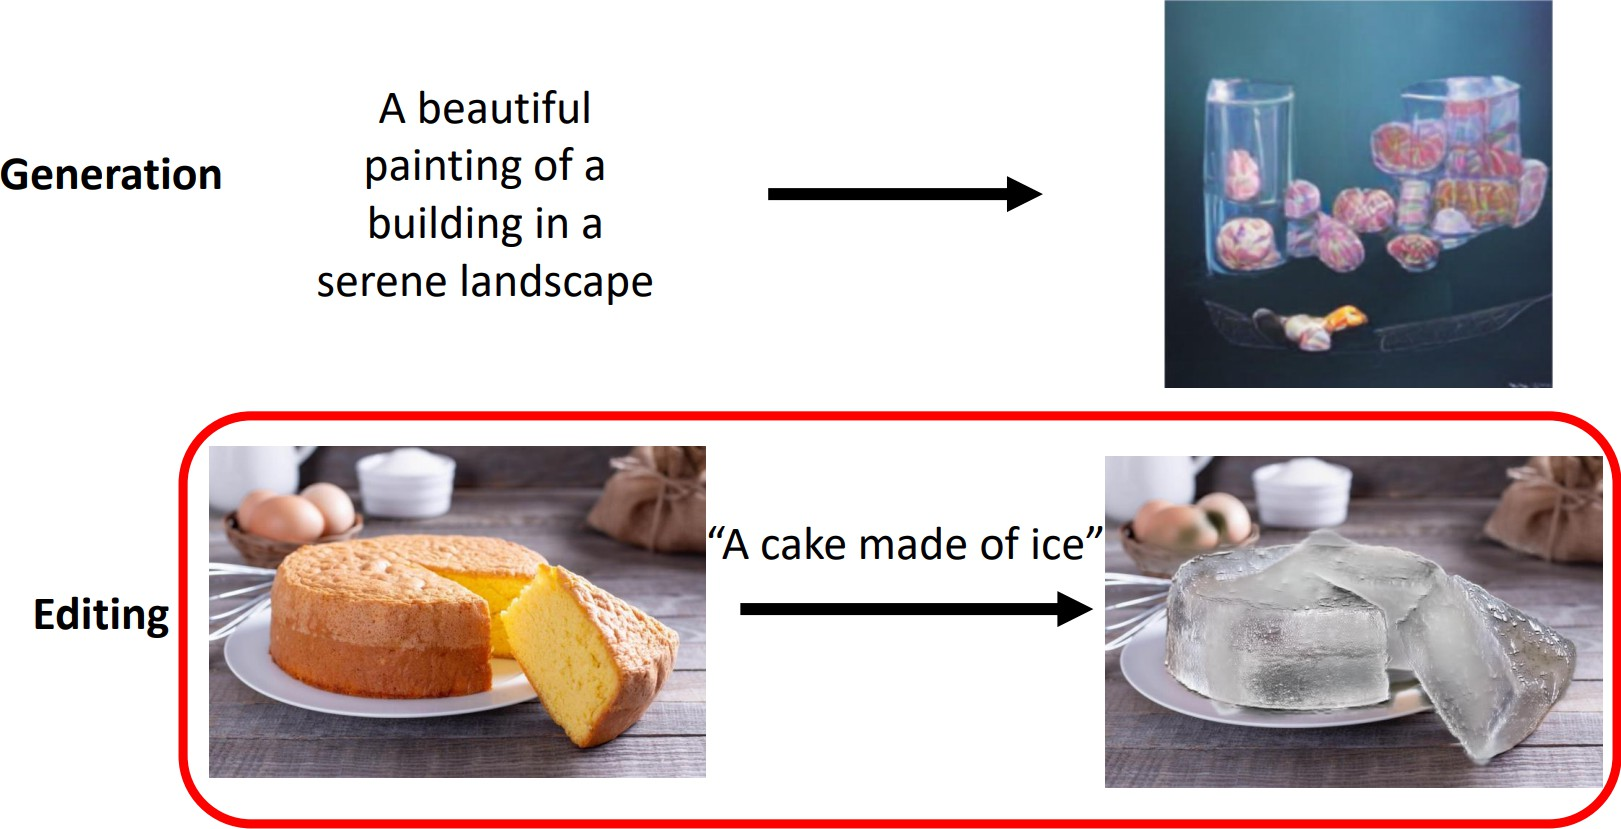
\includegraphics[width=1\textwidth,height=0.9\textheight,keepaspectratio]{images/video/slide_62_1_img.jpg}
    \end{figure}
\end{frame}


\begin{frame}[allowframebreaks]{VQ-GAN + CLIP Editing}
    \large VQ-GAN + CLIP Editing \\[1em]
    \textbf{VQ-GAN + CLIP Editing} combines the strengths of VQ-GAN for image generation and CLIP for text-guided editing, enabling high-quality image synthesis and manipulation.

    \begin{itemize}
        \item \textbf{VQ-GAN:} Generates images from discrete latent codes, allowing for efficient representation.
        \item \textbf{CLIP:} Guides the editing process by understanding text prompts, enabling targeted modifications to generated images.
        \item \textbf{Applications:} Image synthesis, style transfer, and content-aware editing.
    \end{itemize}
\framebreak
    \textbf{How They Work Together:}
    \begin{itemize}
        \item \textbf{Image Generation:} VQ-GAN generates images based on quantized latent codes, while CLIP provides text-based guidance for editing.
        \item \textbf{Text Conditioning:} CLIP's text embeddings condition the VQ-GAN generator, allowing it to produce images that match specific textual descriptions.
        \item \textbf{Loss Function:} The similarity between generated image embeddings and text embeddings from CLIP is used as a loss function to optimize the VQ-GAN generator, ensuring that the generated images align with the given text prompts.
    \end{itemize}
\framebreak
    \begin{figure}
        \centering
        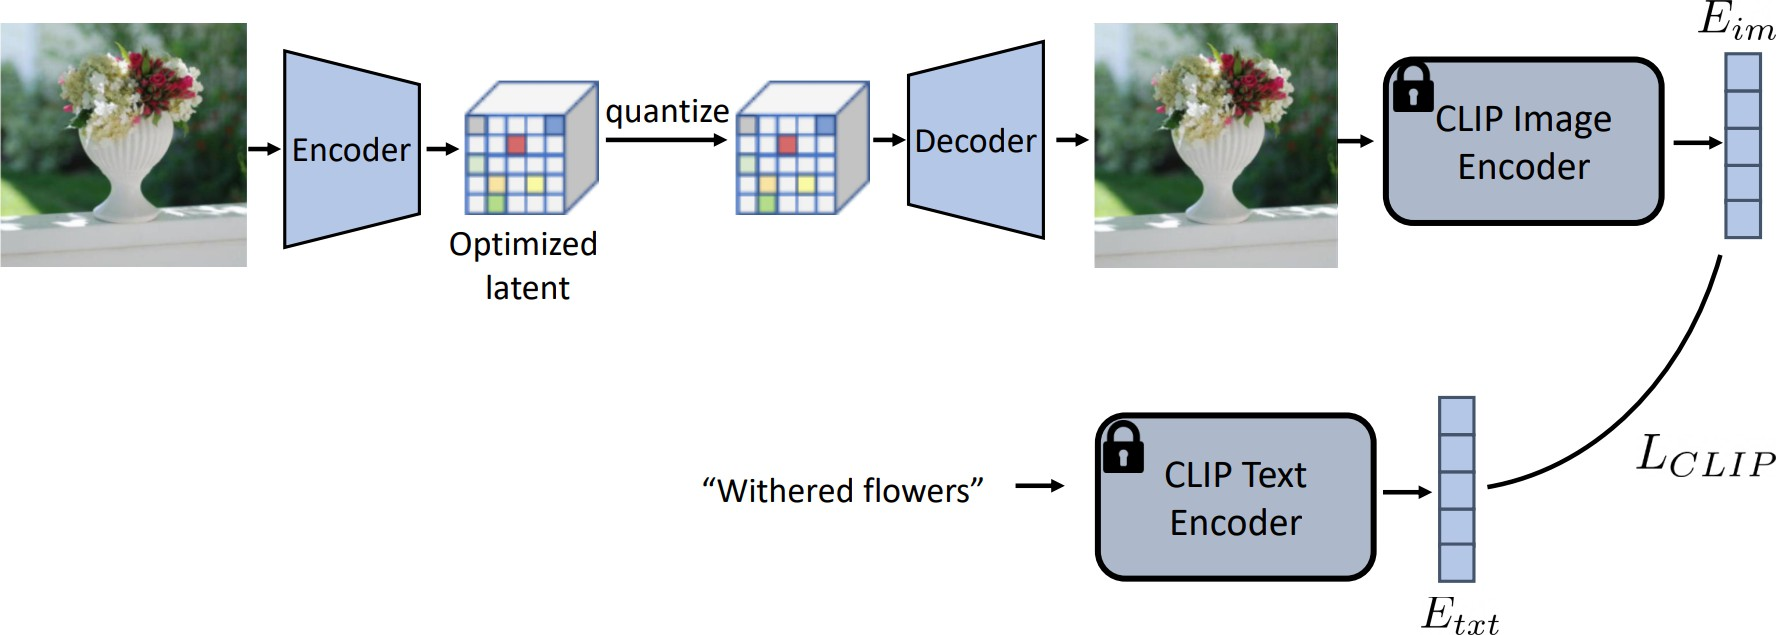
\includegraphics[width=1\textwidth,height=0.8\textheight,keepaspectratio]{images/video/slide_63_1_img.jpg}
    \end{figure}
    {\footnotesize{[VQGAN-CLIP: Open Domain Image Generation and Editing with Natural Language Guidance, Crowson et al. ICCV 13 2021]}}
\framebreak
    \begin{figure}
        \centering
        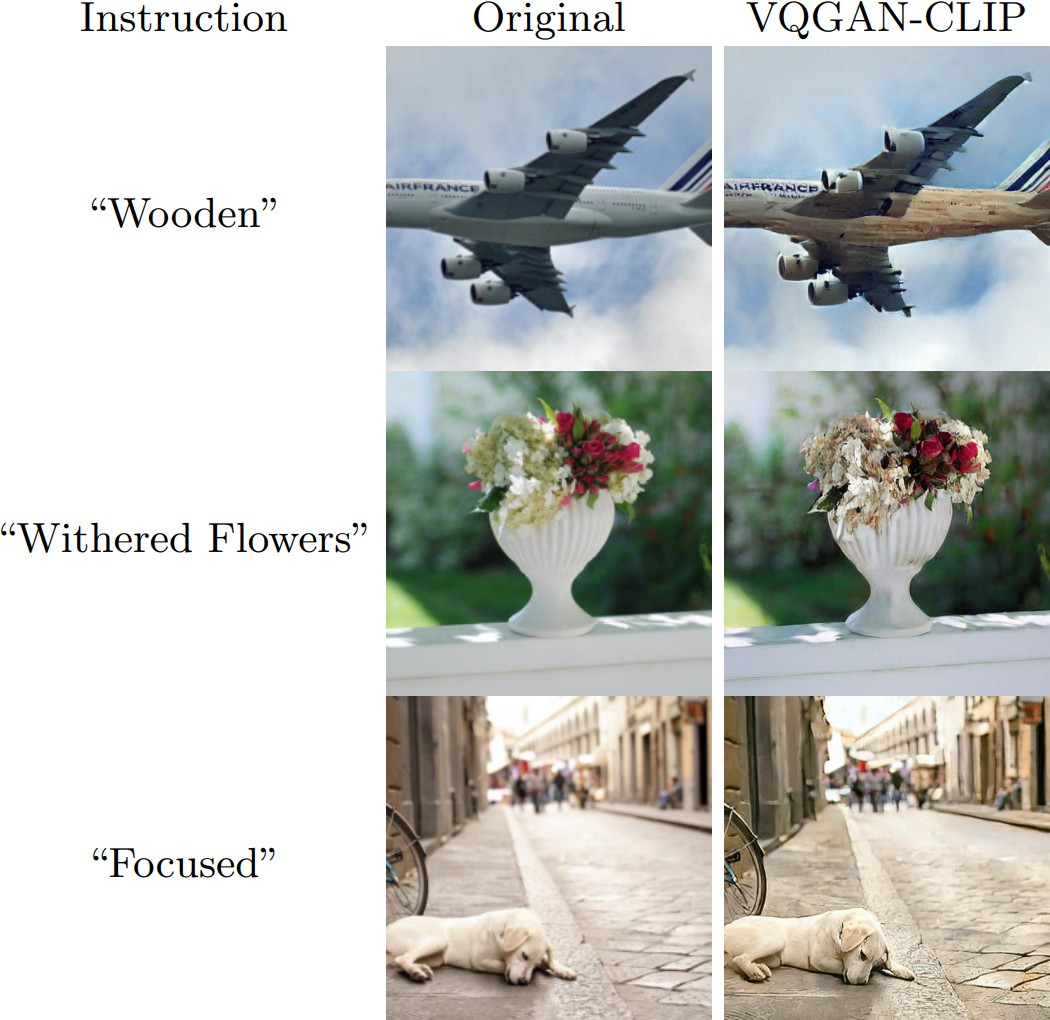
\includegraphics[width=1\textwidth,height=0.9\textheight,keepaspectratio]{images/video/slide_64_1_img.jpg}
    \end{figure}
\end{frame}